%% ENSF 612 Project Proposal (Revised): DupHunter
\documentclass[11pt,a4paper]{article}

\usepackage[left=2cm,right=2cm,top=1.4cm,bottom=1.6cm]{geometry}
\usepackage[T1]{fontenc}
\usepackage{lmodern}
\usepackage{microtype}
\usepackage{booktabs}
\usepackage{tabularx}
\usepackage{array}
\usepackage[table]{xcolor}
\usepackage{tikz}
\usetikzlibrary{arrows.meta}
\usepackage{enumitem}
\usepackage{multicol}
\usepackage{float}
\setlist{nosep,leftmargin=*}
\usepackage[font=small,labelfont=bf,skip=3pt]{caption}
\usepackage{titlesec}
\titlespacing*{\section}{0pt}{6pt}{2pt}
\titleformat*{\section}{\large\bfseries}
\usepackage[colorlinks=true,linkcolor=blue!50!black,citecolor=blue!50!black,urlcolor=blue!50!black]{hyperref}

\setlength{\parskip}{4pt}
\setlength{\parindent}{0pt}
\setlength{\textfloatsep}{6pt}
\setlength{\intextsep}{6pt}
\newcolumntype{Y}{>{\raggedright\arraybackslash}X}
\newcommand{\g}{\cellcolor{blue!22}}
\newcommand{\ms}{\cellcolor{orange!45}}

\begin{document}

\begin{center}
  {\Large\bfseries ENSF~612 Project Proposal (Milestone~1, Revised)}\\[3pt]
  {\small Engineering Large-Scale Data Analytics Systems, Fall 2026\\[1pt]
  Instructor: Dr.~Ebrahim Karami\\[1pt]
  October 26, 2026}
\end{center}


%% ==========================================================================
\section{Project Title}
\textbf{DupHunter: Scalable Duplicate Question Detection on Stack Overflow}

%% ==========================================================================
\section{Group Members}
{\small
\begin{tabularx}{\textwidth}{@{}l Y@{}}
\toprule
\textbf{Name} & \textbf{Main role} \\
\midrule
Satyam Bhanot       & Data pipeline, Spark cluster, scaling study (E8) \\
Iesrat Jahan        & Text representation, MinHash, LSH and its settings (E1, E2, E3) \\
Md Jubayer Khan     & Answer key, evaluation, baselines, SON tag blocking (E5, E6) \\
Navjot Singh Shienh & Checking and ranking candidates, handling oversized LSH buckets (E4, E7) \\
\bottomrule
\end{tabularx}}

%% ==========================================================================
\section{Problem Statement}

Stack Overflow is a website where programmers ask and answer questions. Many
new questions have already been asked before, just in different words. These
are called \emph{duplicates}. Today, volunteers find and close them by hand,
and many are missed.

We want to build a system that finds duplicate questions automatically. The
hard part is size. Stack Overflow has about 24 million questions, and comparing
every question with every other one would take years on one computer. We need
methods built for large data that can run on more than one machine.

\textbf{One problem, studied in depth.} After feedback on our first proposal,
we dropped the AI-impact study and the streaming check, which were only loosely
tied to duplicate detection. We use that time to go deeper into the duplicate
search itself. Each stage of the system is a design choice, and each choice is
settled by an experiment (E1 to E8 in Table~\ref{tab:exp}).

\textbf{Questions we want to answer:}
\begin{enumerate}[label=\textbf{Q\arabic*.},leftmargin=2.2em]
  \item \textbf{(Core)} How many known duplicates can our MinHash and LSH
        system find, and how close does it come to an exact search that checks
        every pair?
  \item \textbf{(Core)} Do MinHash and LSH behave the way the course theory
        predicts on real questions, and which settings give the best balance
        between missed duplicates and wasted work?
  \item \textbf{(Core)} What slows the system down as it grows (oversized
        buckets, data moved between machines, memory), and how does run time
        change with more cores, a second machine, and more data?
  \item Does grouping questions by frequent tag sets, found with SON, save work
        without losing many duplicates?
\end{enumerate}

\textbf{Expected outcome:} a working Spark system for duplicate search, and
eight experiments that explain each design choice and its cost.

%% ==========================================================================
\section{Motivation and Application}

Duplicate questions waste time. People wait for answers that already exist,
experts answer the same thing again, and volunteers spend hours searching. A
tool that finds duplicates could show a user an existing answer before they
post. The same kind of search is used to remove repeated pages from web search,
to catch copied documents, and to clean AI training data.

At this size, a good algorithm is not enough: the data must be spread over
machines, common phrases can overload one machine, and every setting trades
accuracy against work. This is what ENSF~612 teaches: MapReduce and Spark,
shingling, MinHash, LSH, and frequent itemsets~\cite{mmds}.

%% ==========================================================================
\section{Dataset}

\textbf{Source.} We will use the public Stack Exchange data dump on the Internet
Archive (\url{https://archive.org/details/stackexchange}). The newest release
is from September 30, 2026~\cite{sedump}. It is free to use under the
CC~BY-SA~4.0 license.

\textbf{Size and format.} The Stack Overflow archive is a single 64.2\,GiB
(68.9\,GB) compressed file (\texttt{.7z}) covering July 2008 to September 2026.
Inside, each table is an XML file with one record per line. We only need the
columns in Table~\ref{tab:data} and skip every other table. Record counts are estimates from older
releases; we will update them after loading the data.

\begin{table}[H]
\centering
\caption{The data we will use.}
\label{tab:data}
\small
\begin{tabularx}{\textwidth}{@{}l l Y Y@{}}
\toprule
\textbf{Table} & \textbf{Records (approx.)} & \textbf{Fields we keep} & \textbf{What we use it for} \\
\midrule
Posts     & 60 million (24 million questions) & id, type, title, body, tags, date & Question text, tags, and dates \\
PostLinks & 10 million & post id, related post id, link type & Known duplicate pairs (our answer key) \\
\bottomrule
\end{tabularx}
\end{table}

\textbf{How much data we will use.}
\begin{itemize}
  \item Our main runs use questions tagged \texttt{python} (roughly 2 million;
        we will confirm the count). This is still large: 2 million questions
        make about 2 trillion pairs. We only score duplicate pairs where both
        questions are in the subset.
  \item If time allows, we run the final system on all 24 million questions to
        see how it behaves on data more than ten times larger.
  \item We build and debug everything on the Super User site first (1.4\,GB
        compressed, same format, about 50 times smaller).
\end{itemize}

\textbf{Data quality and limitations.}
\begin{itemize}
  \item Question text is stored as HTML, with code mixed into the writing.
  \item Deleted posts are missing.
  \item Not every duplicate was marked by volunteers, so our answer key is
        incomplete and our precision will be a lower bound.
  \item Some duplicates share few words with their original. Before building
        anything, we measure how similar known duplicate pairs really are
        compared with random pairs (E1), so we know what the search must find.
  \item Results on one tag may not hold for every topic.
\end{itemize}

\textbf{Preprocessing.} We extract only the two tables and read them as a
stream, so we never store hundreds of GB of unpacked XML. We keep the needed
columns and save them as Parquet (a compressed table format that Spark reads
quickly), split by year. For each question, we remove HTML tags, keep code
blocks separate, and break the text into short groups of words called
\emph{shingles}.

%% ==========================================================================
\section{Proposed Methodology}

\begin{figure}[H]
\centering
\resizebox{\textwidth}{!}{%
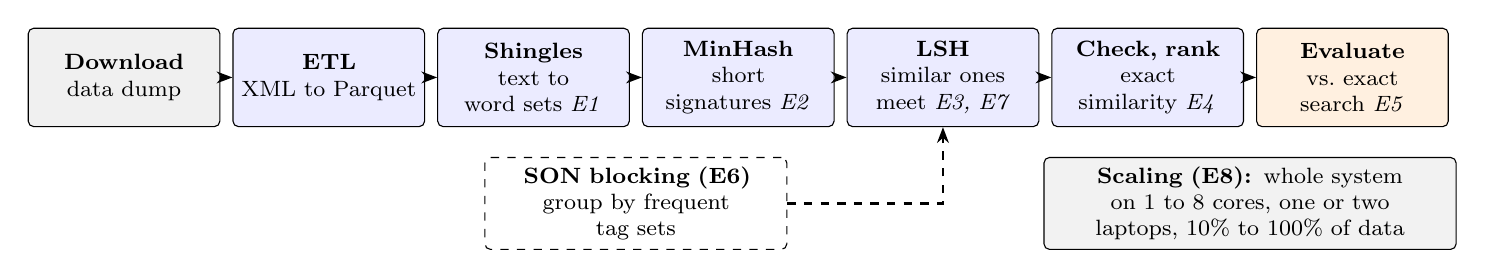
\begin{tikzpicture}[
  box/.style={draw, rounded corners=2pt, align=center, font=\footnotesize, text width=2.2cm, minimum height=1.25cm, fill=blue!8},
  side/.style={box, dashed, fill=white},
  arr/.style={-{Stealth[length=2mm]}, thick},
  darr/.style={-{Stealth[length=2mm]}, thick, dashed}
]
\node[box, fill=gray!12] (a) at (0,0)    {\textbf{Download}\\ data dump};
\node[box]               (b) at (2.6,0)  {\textbf{ETL}\\ XML to Parquet};
\node[box]               (c) at (5.2,0)  {\textbf{Shingles}\\ text to\\ word sets \textit{E1}};
\node[box]               (d) at (7.8,0)  {\textbf{MinHash}\\ short\\ signatures \textit{E2}};
\node[box]               (e) at (10.4,0) {\textbf{LSH}\\ similar ones\\ meet \textit{E3, E7}};
\node[box]               (f) at (13.0,0) {\textbf{Check, rank}\\ exact\\ similarity \textit{E4}};
\node[box, fill=orange!12] (g) at (15.6,0) {\textbf{Evaluate}\\ vs.\ exact\\ search \textit{E5}};
\draw[arr] (a) -- (b); \draw[arr] (b) -- (c); \draw[arr] (c) -- (d); \draw[arr] (d) -- (e); \draw[arr] (e) -- (f); \draw[arr] (f) -- (g);
\node[side, text width=3.6cm, minimum height=0.9cm] (s) at (6.5,-1.6) {\textbf{SON blocking (E6)}\\ group by frequent\\ tag sets};
\draw[darr] (s.east) -| (e.south);
\node[draw, rounded corners=2pt, fill=gray!10, font=\footnotesize, align=center, text width=5.0cm, minimum height=0.9cm] (z) at (14.3,-1.6)
  {\textbf{Scaling (E8):} whole system on 1 to 8 cores, one or two laptops, 10\% to 100\% of data};
\end{tikzpicture}}
\caption{DupHunter. Each stage is a design choice tested by the experiment named in it. The dashed box is the secondary part.}
\label{fig:pipeline}
\end{figure}

\textbf{The core.} We turn each question into a set of shingles and compress
it into a short MinHash \emph{signature}. LSH cuts each signature into bands;
questions that match on a whole band land in the same bucket, and we only
compare questions that share a bucket. We then check each candidate pair with
its exact similarity and rank the candidates for each question. All of these
are our own Spark code, written in the MapReduce style~\cite{dean2004}.

\begin{table}[!t]
\centering
\caption{Experiments. Each one settles a design choice or measures a cost.}
\label{tab:exp}
\small
\begin{tabularx}{\textwidth}{@{}l l Y Y l@{}}
\toprule
\textbf{Exp.} & \textbf{Stage} & \textbf{What we compare} & \textbf{What we measure} & \textbf{Q} \\
\midrule
E1 & Shingles & Word groups of 1 to 5 words vs.\ character groups; title only vs.\ title and body; with and without very common shingles (boilerplate code) & How well real duplicates stand apart from random pairs & Q1 \\
E2 & MinHash & Signatures of 32 to 256 numbers & Error of the similarity estimate vs.\ the error theory predicts; time and memory & Q2 \\
E3 & LSH & Several band and row settings & Measured S-curve vs.\ the one theory predicts; recall vs.\ number of candidates & Q1, Q2 \\
E4 & Check and rank & Ranking by signature alone vs.\ exact similarity vs.\ TF-IDF re-ranking & Recall@K, Precision@K, MAP, NDCG & Q1 \\
E5 & Baselines & Exact search of every pair on a sample; Spark's built-in \texttt{MinHashLSH} & Accuracy given up for the time saved & Q1 \\
E6 & Blocking & No blocking vs.\ single tags vs.\ SON frequent tag sets & Run time, data moved, recall lost & Q4 \\
E7 & Big buckets & Size limit vs.\ splitting big buckets over many tasks vs.\ dropping common shingles & Time of the slowest task, recall, memory & Q3 \\
E8 & Scaling & Table~\ref{tab:scale} & Run time, speedup, data moved, peak memory & Q3 \\
\bottomrule
\end{tabularx}
\end{table}

\textbf{How we will evaluate.} Accuracy uses Recall@K, Precision@K, MAP, and
NDCG (how high the real duplicate is ranked), plus the reduction ratio (the
share of pairs we never compare). We also break recall down by similarity,
tag, question length, and year, to see where and why the system fails. For
speed we record run time, speedup (how many times faster than one core),
data moved between machines, peak memory, and the time of the slowest task.
Each scaling setting runs three times.

\textbf{Compute setup.} We have two laptops with 16\,GB of RAM each. Laptop~A
has an Intel Core i7-13650HX (14 cores) and Laptop~B an AMD Ryzen~7 5800H
(8 cores). Both run Windows, so Spark and HDFS run inside WSL2 (Linux on
Windows). We connect them as a Spark standalone cluster~\cite{zaharia2012} on
the same wired network: Laptop~A runs the master, the driver, and one worker;
Laptop~B runs one worker. Each worker gives Spark 8 cores and about 8\,GB of
memory (7\,GB on Laptop~B, which has 13.9\,GB usable). The data is stored in
HDFS~\cite{hdfs} with a copy on each laptop, so every worker reads from its own
disk. Spark runs tasks inside \emph{executors}, its worker processes. For the
1, 2, 4, and 8 worker tests we give one executor 1, 2, 4, and then 8 cores,
because each extra executor needs its own memory and eight would not fit in
16\,GB. MinHash signatures for 2 million questions need only about 1\,GB.

\begin{table}[H]
\centering
\caption{Scaling tests (E8) on the two-laptop cluster.}
\label{tab:scale}
\small
\begin{tabularx}{\textwidth}{@{}l Y Y@{}}
\toprule
\textbf{Test} & \textbf{Setup} & \textbf{What it shows} \\
\midrule
A. More cores & 1, 2, 4, and 8 cores on Laptop~B, whose 8 cores are all the same; same data & Speedup, and how much of the work cannot run in parallel \\
B. Second machine & 8 cores on A alone, on B alone, 4 + 4 on both, then 8 + 8 & The cost of the network, and how the slower laptop holds back the faster one \\
C. More data & 10\%, 25\%, 50\%, and 100\% of the subset; all of Stack Overflow if time allows & How run time and memory grow with data size \\
\bottomrule
\end{tabularx}
\end{table}

\textbf{Priority and cut order.} Q1 to Q3 must be finished. If time runs short,
we cut, in this order: the run on all of Stack Overflow, splitting big buckets
(we keep the simple size limit), TF-IDF re-ranking, and SON blocking (Q4).
Even after these cuts, every member still has core results.

%% ==========================================================================
\section{Algorithms and Techniques}

We write the course algorithms ourselves. Exact search on a sample, Spark's
\texttt{MinHashLSH}, and Spark's \texttt{FPGrowth} are used only for comparison,
so the report clearly shows which code is ours.
\begin{itemize}
  \item \textbf{Core, our own code:} shingling with removal of very common
        shingles (E1); MinHash~\cite{broder1997} (E2); LSH
        banding~\cite{indyk1998} (E3); exact checking and ranking of candidates
        (E4); handling of big buckets~\cite{kwon2012} (E7); all as Spark jobs in
        the MapReduce style~\cite{dean2004} (E8).
  \item \textbf{Secondary:} SON frequent itemsets~\cite{son1995} for tag
        blocking (E6).
  \item \textbf{Stretch:} TF-IDF re-ranking~\cite{mmds} (E4), splitting big
        buckets over many tasks (E7), and the run on all of Stack Overflow (E8).
\end{itemize}

%% ==========================================================================
\section{Expected Challenges}
{\small
\begin{tabularx}{\textwidth}{@{}>{\raggedright\arraybackslash}p{6.6cm} Y@{}}
\toprule
\textbf{Challenge} & \textbf{How we plan to handle it} \\
\midrule
Duplicates written in very different words & Measure it first (E1); report recall by similarity level \\
Missing duplicate labels & Treat precision as a lower bound; rely mainly on recall and ranking \\
A few huge buckets (common phrases) make one task much slower & Measure the slowest task; compare a size limit with splitting buckets (E7) \\
Choosing LSH settings & Compare measured results with theory on Super User first (E3) \\
Moving data between laptops; 16\,GB of memory each & Wired network; process bands in batches; keep only needed columns \\
Two different laptops (Intel and AMD) & Time each one alone first (test B), so the gap is measured, not hidden \\
Blocking misses duplicates with different tags & Measure the recall lost compared with no blocking (E6) \\
\bottomrule
\end{tabularx}}

%% ==========================================================================
\section{Expected Results}
\begin{itemize}
  \item \textbf{Q1:} LSH will find most known duplicates while skipping more
        than 99.9\% of all pairs; exact checking will rank the real duplicate
        higher, close to Spark's built-in version.
  \item \textbf{Q2:} the measured match rates will follow the theory closely,
        and 128 numbers per signature will be enough.
  \item \textbf{Q3:} MinHash will speed up almost in line with the number of
        cores, because it needs no communication. LSH will speed up less,
        because data must move between machines and a few big buckets slow it
        down; splitting those buckets will shorten the slowest task.
  \item \textbf{Q4:} tag blocking will cut run time and data moved, with a
        small loss in recall.
\end{itemize}

%% ==========================================================================
\section{Initial Project Schedule}

The core comes first. On November 13 we check progress and decide which stretch
parts go ahead.

\begin{table}[H]
\centering
\caption{Weekly plan (blue: main work; orange: milestone).}
\label{tab:plan}
\footnotesize
\setlength{\tabcolsep}{3pt}
\begin{tabularx}{\textwidth}{@{}Y l *{6}{>{\centering\arraybackslash}p{1.3cm}}}
\toprule
\textbf{Task (week starting)} & \textbf{Who} & \textbf{Oct 26} & \textbf{Nov 2} & \textbf{Nov 9} & \textbf{Nov 16} & \textbf{Nov 23} & \textbf{Nov 30} \\
\midrule
Download, ETL, cluster setup                  & Satyam  & \g & \g &  &  &  &  \\
Shingles, MinHash, LSH (E1, E2, E3)           & Iesrat  & \g & \g & \g &  &  &  \\
Answer key, evaluation, baselines (E5)        & Jubayer &  & \g & \g &  &  &  \\
Checking candidates, big buckets (E4, E7)     & Navjot  &  & \g & \g & \g &  &  \\
Core checkpoint                               & All     &  &  & \ms Nov 13 &  &  &  \\
Scaling study (E8)                            & Satyam  &  &  & \g & \g &  &  \\
SON tag blocking (E6)                         & Jubayer &  &  & \g & \g &  &  \\
Results freeze                                & All     &  &  &  & \ms Nov 20 &  &  \\
Presentation                                  & All     &  &  &  & \g & \g &  \\
Final report and code                         & All     &  &  &  &  & \g & \ms Dec 4 \\
\bottomrule
\end{tabularx}
\end{table}

%% ==========================================================================
\section{References}
\vspace{-14pt}
\begin{multicols}{2}
{\footnotesize
\renewcommand{\section}[2]{}
\begin{thebibliography}{99}
\setlength{\itemsep}{0pt}
\setlength{\parskip}{0pt}
\bibitem{mmds} A.~Rajaraman and J.~D.~Ullman, \emph{Mining of Massive Datasets}. Cambridge University Press, 2011.
\bibitem{sedump} Stack Exchange, Inc., ``Stack Exchange Data Dump 2026-09-30,'' Internet Archive, \url{https://archive.org/details/stackexchange_20260930}.
\bibitem{dean2004} J.~Dean and S.~Ghemawat, ``MapReduce: Simplified data processing on large clusters,'' in \emph{Proc. OSDI}, 2004.
\bibitem{zaharia2012} M.~Zaharia \emph{et al.}, ``Resilient distributed datasets: A fault-tolerant abstraction for in-memory cluster computing,'' in \emph{Proc. NSDI}, 2012.
\bibitem{broder1997} A.~Z.~Broder, ``On the resemblance and containment of documents,'' in \emph{Proc. Compression and Complexity of Sequences}, 1997.
\bibitem{indyk1998} P.~Indyk and R.~Motwani, ``Approximate nearest neighbors: Towards removing the curse of dimensionality,'' in \emph{Proc. ACM STOC}, 1998.
\bibitem{son1995} A.~Savasere, E.~Omiecinski, and S.~Navathe, ``An efficient algorithm for mining association rules in large databases,'' in \emph{Proc. VLDB}, 1995.
\bibitem{hdfs} K.~Shvachko, H.~Kuang, S.~Radia, and R.~Chansler, ``The Hadoop distributed file system,'' in \emph{Proc. IEEE MSST}, 2010.
\bibitem{kwon2012} Y.~Kwon, M.~Balazinska, B.~Howe, and J.~Rolia, ``SkewTune: Mitigating skew in MapReduce applications,'' in \emph{Proc. ACM SIGMOD}, 2012.
\end{thebibliography}}
\end{multicols}

\end{document}
